% 
% EXERCICIOS DO TEMA 0.- INTRODUCCIÓN
%
% Repaso de conceptos de Perspectivas sobre a música

\section{Pensamentos, teorías e perspectivas sobre a música}

\begin{ejercicio}[Perspectivas sobre música- Rene Descartes]

% Ilustramos os exercicios con figuras
% --- Rene Descartes:
\begin{wrapfigure}{l}{0.30\textwidth} 
\begin{center} 
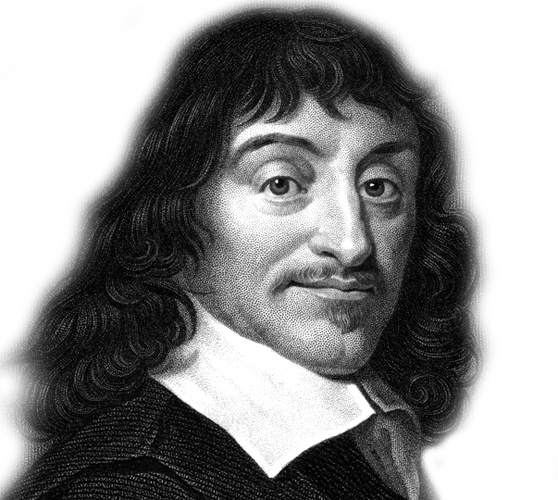
\includegraphics[width=0.20\textwidth]{/ud-00/descartes.png} 
\end{center} 
\caption{\\ \textbf{Rene Descartes} \\ 
Francia, 1596 - Suecia, 1650} 
\label{fig:descartes}
\end{wrapfigure}
% ---

As perspectivas sobre a música varian ao longo das diferentes épocas da historia. 
Algunhas reflexións, convidan a pensar na música como unha arte totalmente ligada a expresión de sentimentos; outras xustifican que, a música hai que considerala unha ciencia.

Desde os inicios da música, os teóricos, filósofos, músicos e grandes ilustrados trataron de comprender o feito musical e establecer relacións que lles axudasen a coñecer mellor o seu significado. É o caso de Pitágoras, Descartes, Kant, Wagner e moitos outros, que coas súas reflexións e perspectivas sobre a música sentan os precedentes do pensamento estétilo e musical, dentro da Historia do pensamento musical. 

Descartes s. {\scriptsize  XVII} define a música do seguinte xeito:

    \begin{quotation}{\small
     \noindent
     A mesma cousa que a uns invita a bailar a outros pode facer chorar. Pois isto non provén senón da asociación de ideas na nosa mente; como aqueles que algunha vez se divertiron bailando con certa peza, tan pronto como a volvan a escoltar volverán ás ganas de bailar; pola contra, se algún só oíu gallardas cando lle aconteceu algo malo, volverá  a entristecerse cando as escoite de novo.}
    \end{quotation}
 
\begin{enumerate}[1)]
 \item 
 Que perspectiva sobre a música adoita Descartes segundo a afirmación anterior?
 \begin{enumerate}[a)]
  \item 
  Música como expresión dos sentimentos
  \item
  Música como arte
  \item %\label{sol:1}
  Música como feito musical
  \item
  Ningunha das anteriores
 \end{enumerate}
 \item 
 A quen atribúes a seguinte afirmación? \dotfill
     \begin{quote}
    {\small
    Os números son as cousas; agora ben, a música é número. O mundo é música; o cosmos é unha lira sublime de sete cordas.
    }
    \end{quote}
\end{enumerate}

\end{ejercicio}

% --------------------------

\begin{ejercicio}[Perspectivas sobre música - Richard Wagner]

% Ilustramos os exercicios con figuras
% --- Richard Wagner:
\begin{wrapfigure}{r}{0.30\textwidth} 
\begin{center} 
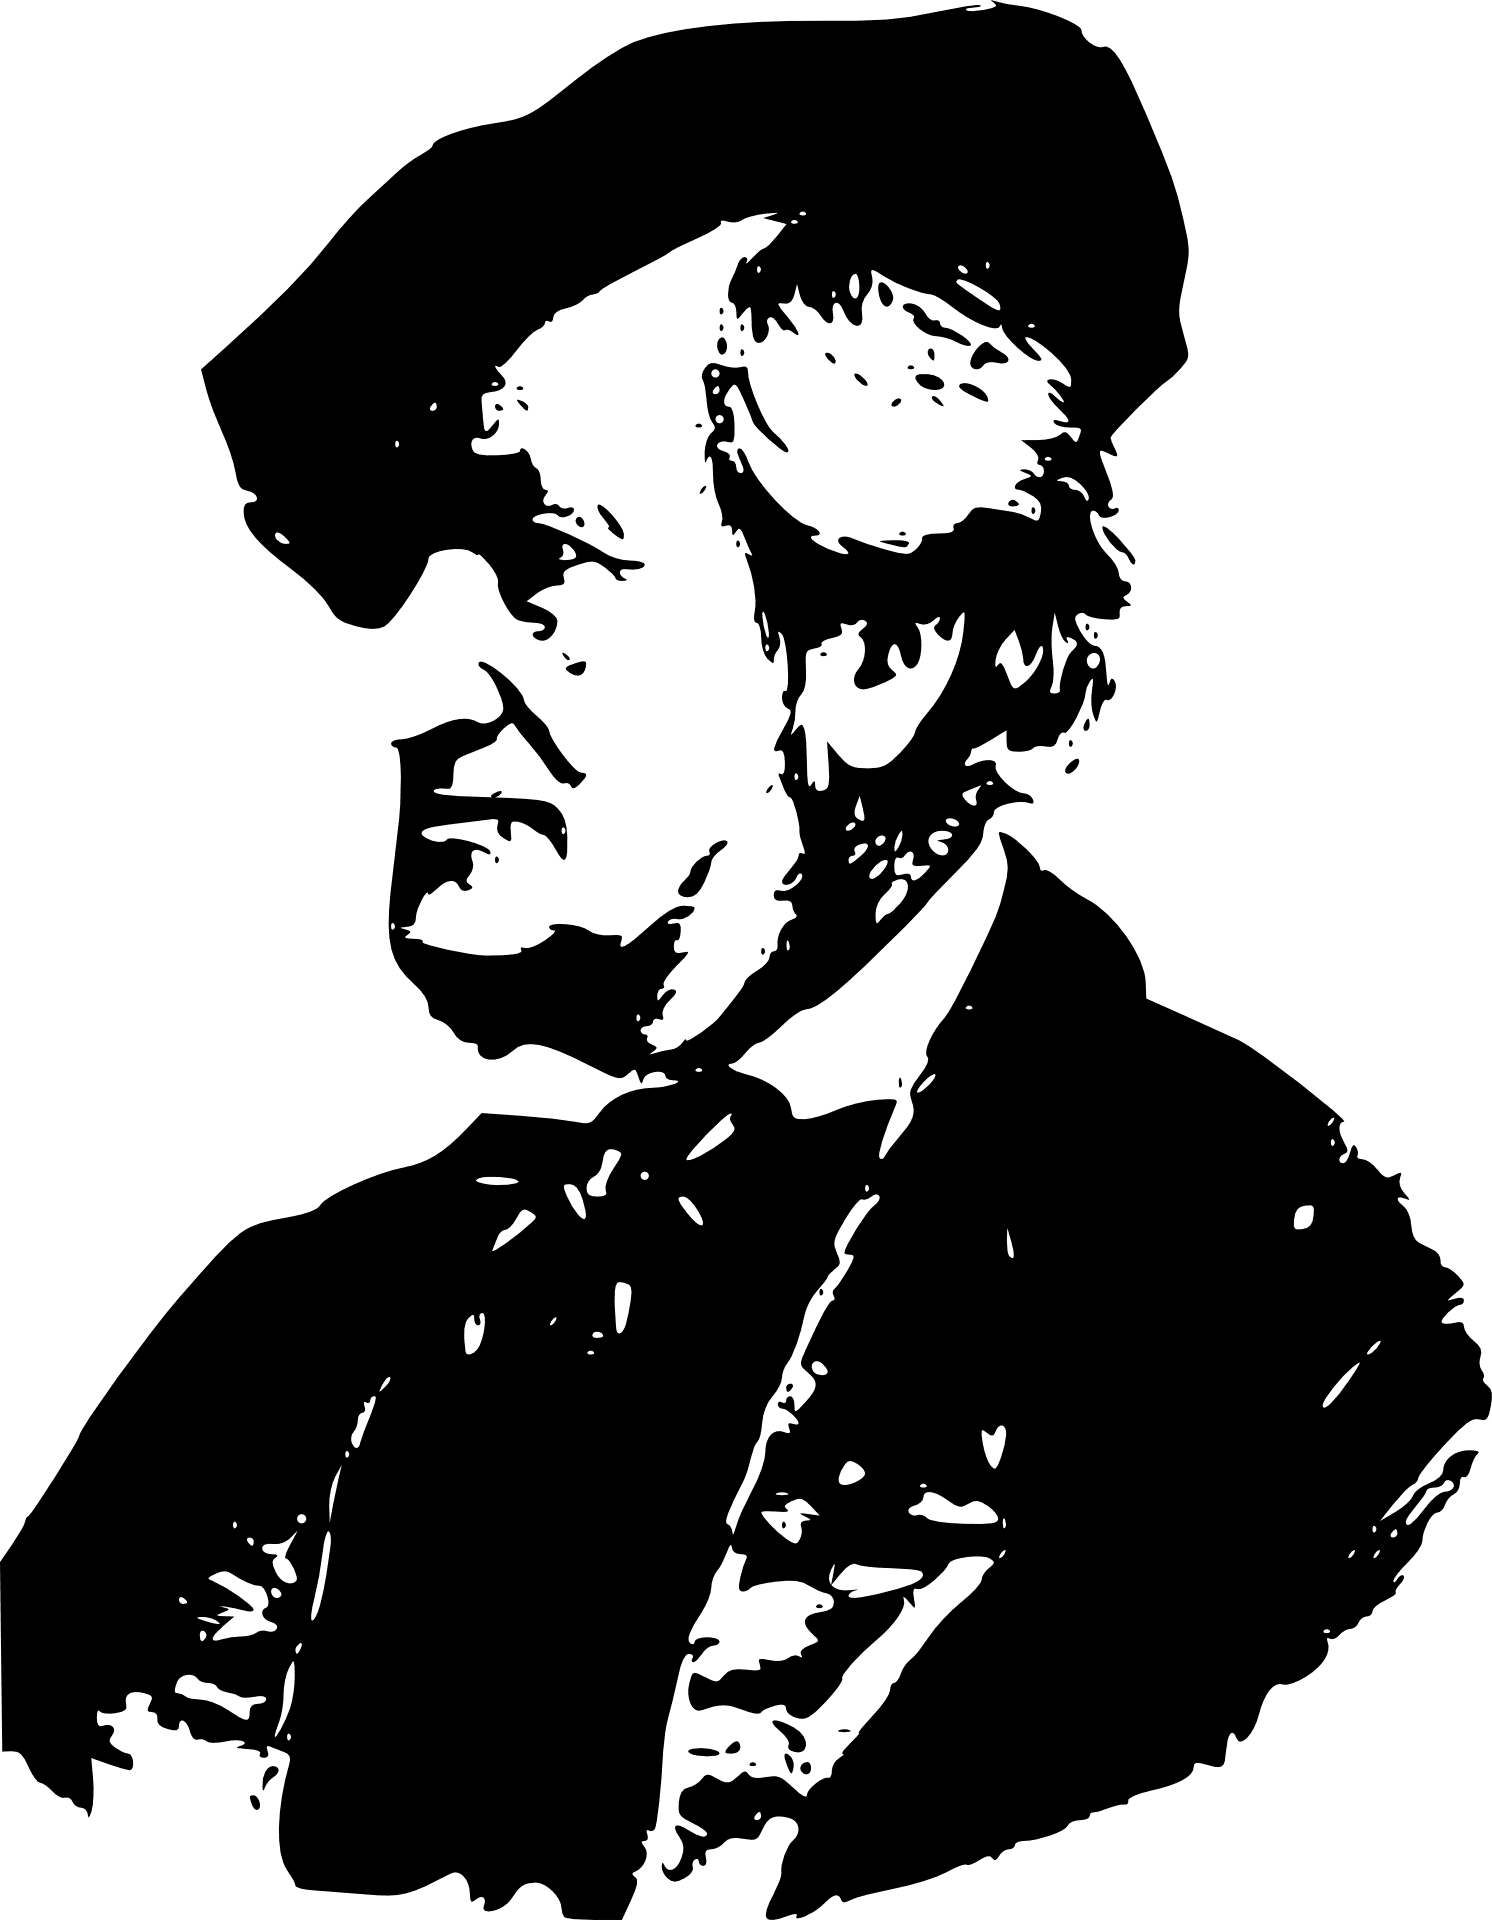
\includegraphics[width=0.20\textwidth]{/ud-00/wagner.png} 
\end{center} 
\caption{\\ \textbf{Richard Wagner} \\ 
Leipzig, 1813 - Venecia, 1883} 
\label{fig:wagner}
\end{wrapfigure}
% ---

Wilhelm Richard Wagner (Leipzig, 22 de maio de 1813 - Venecia, 13 de febreiro de 1883) foi un compositor, director de orquestra, poeta, ensaísta, dramaturgo e teórico musical alemán do Romanticismo.

Unha das súas maiores achegas á música foi o cambio de perspectiva acerca das composicións, que Wagner consideraba como ``obras de arte totais'' nas que sintetizaban todas as grandes artes: visuais, poéticas, escénicas, musicais, \ldots

Foi un dos máximos expoñentes do romanticismo musical alemán, que rompeu cos moldes canónicos do clasicismo. 
No s.{\scriptsize XIX}, Richard Wagner afirmaba sobre a música:

    \begin{quotation}{\small
     \noindent
     O son vén do corazón e a súa linguaxe artística natural é a música. A melodía é a lingua absoluta, a través da que o músico fala a todos os corazóns.}
    \end{quotation}
 
\begin{enumerate}[1)]
 \item 
 Que perspectiva sobre a música adoita Wagner segundo a afirmación anterior?
 \begin{enumerate}[a)]
  \item 
  Música como expresión dos sentimentos
  \item %\label{sol:2}
  Música como arte
  \item 
  Música como feito musical
  \item
  Ningunha das anteriores
 \end{enumerate}
 \item 
 A quen atribúes a seguinte afirmación sobre a música? \dotfill
     \begin{quote}
    {%\small
    [\ldots] a arte educativa por excelencia que se insire na alma e forma a virtude
    }
    \end{quote}
\end{enumerate}
\end{ejercicio}

% ------

\begin{ejercicio}[Teorías sobre a orixe da música]
Sinala a opción correcta, segundo as afirmacións que se indican nos seguintes puntos.
\begin{enumerate}[1)]
 \item 
 As teorías logoxénicas consideran que a música naceu asociada á linguaxe comunicativa.
  \begin{enumerate}[a)]
   \item %\label{sol:3}
   verdadeiro, nace da necesidade de comunicación
   \item 
   falso, tiñan unha función máxico-relixiosa
  \end{enumerate}
  \item
  Que teorías postulan que o corpo humano é un instrumento en si mesmo? 
  \begin{enumerate}[a)]
   \item 
   teorías logoxénicas
   \item 
   teorías máxico-relixiosas
   \item %\label{sol:4}
   teorías quinéticas
   \item 
   teorías conspirativas
  \end{enumerate}
 \end{enumerate}

\end{ejercicio}



